\begin{figure}[H]
\centering

\includegraphics[width=\textwidth]{实验报告10-2025051923.png}
% \caption{}
\label{}
\end{figure}

\section{二叉链表树实验}

(1) 复制一棵二叉树。
(2) 判断两棵二叉树是否相似。

\begin{figure}[H]
\centering
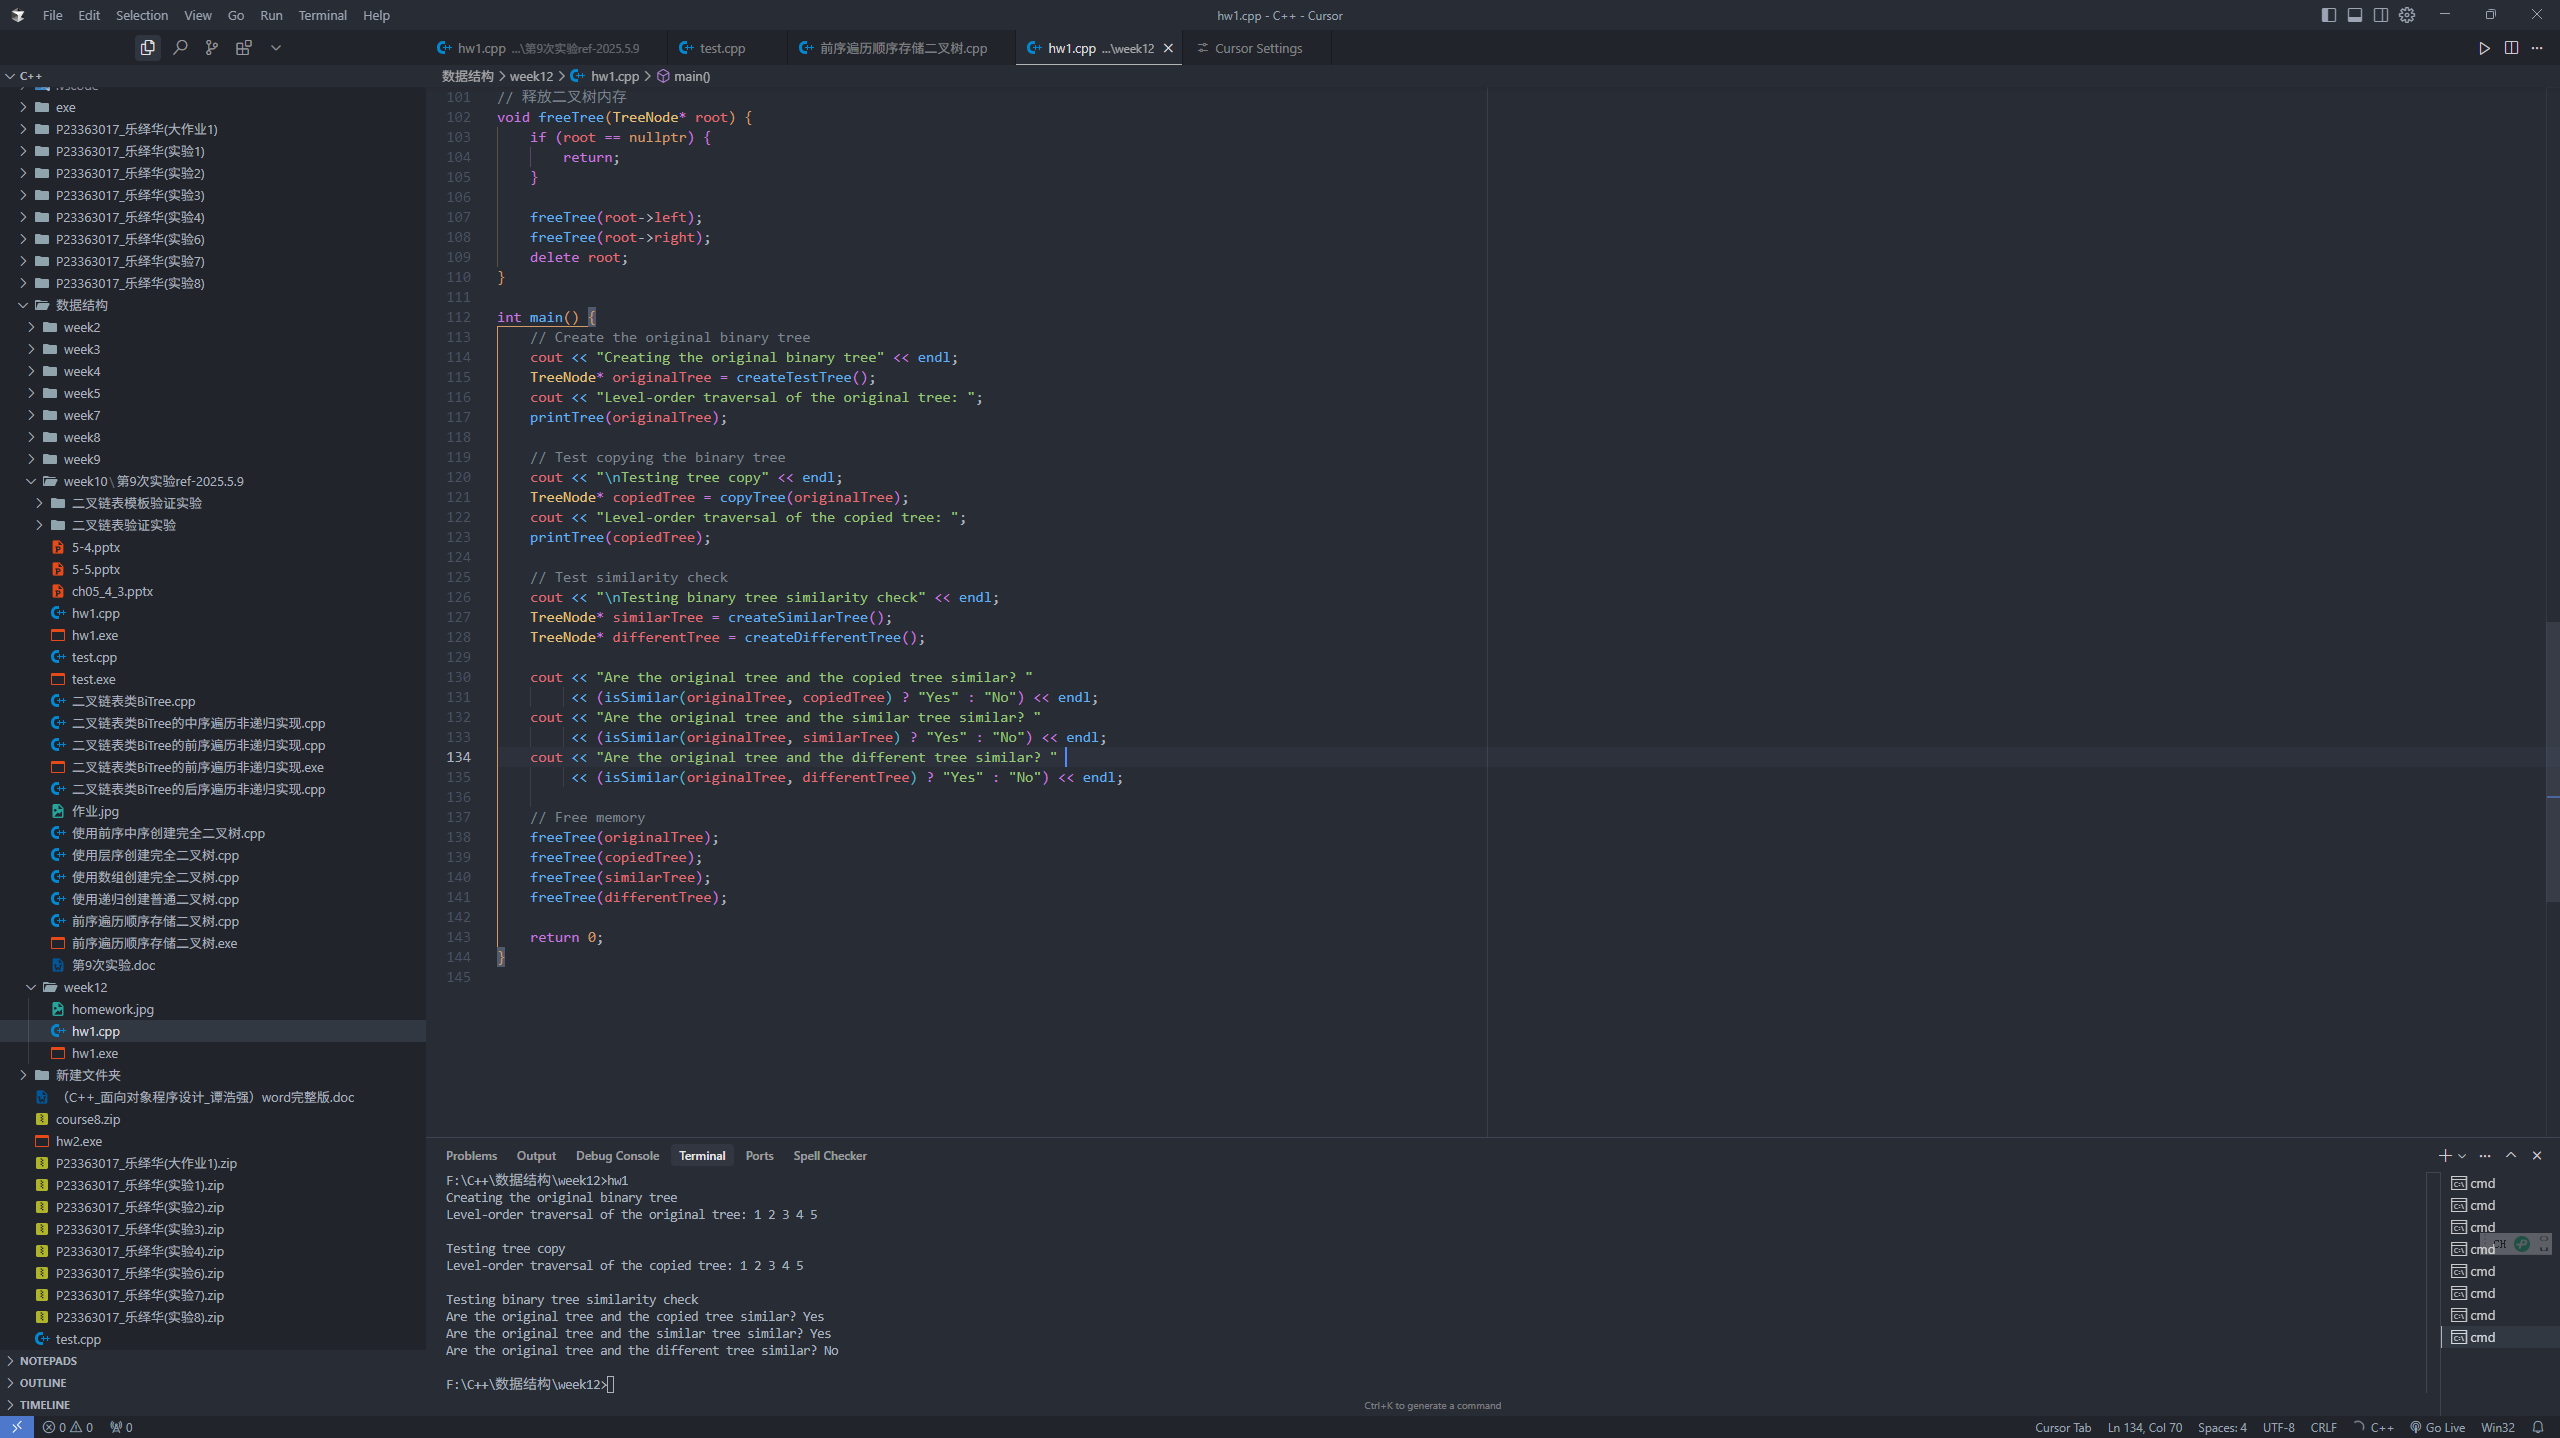
\includegraphics[width=\textwidth]{1-实验报告10-2025051923.png}
% \caption{}
\label{}
\end{figure}

\begin{lstlisting}[language=C++]

#include <iostream>

using namespace std;

  

// 二叉树节点定义

struct TreeNode {

    int data;

    TreeNode* left;

    TreeNode* right;

    TreeNode(int val) : data(val), left(nullptr), right(nullptr) {}

};

  

// 复制二叉树

TreeNode* copyTree(TreeNode* root) {

    if (root == nullptr) {

        return nullptr;

    }

    // 创建新节点

    TreeNode* newNode = new TreeNode(root->data);

    // 递归复制左右子树

    newNode->left = copyTree(root->left);

    newNode->right = copyTree(root->right);

    return newNode;

}

  

// 判断两棵二叉树是否相似

bool isSimilar(TreeNode* root1, TreeNode* root2) {

    // 两棵树都为空,认为相似

    if (root1 == nullptr && root2 == nullptr) {

        return true;

    }

    // 一棵树为空,另一棵不为空,不相似

    if (root1 == nullptr || root2 == nullptr) {

        return false;

    }

    // 递归判断左右子树是否相似

    return isSimilar(root1->left, root2->left) &&

           isSimilar(root1->right, root2->right);

}

  

// 创建一棵测试二叉树

TreeNode* createTestTree() {

    TreeNode* root = new TreeNode(1);

    root->left = new TreeNode(2);

    root->right = new TreeNode(3);

    root->left->left = new TreeNode(4);

    root->left->right = new TreeNode(5);

    return root;

}

  

// 创建另一棵相似但值不同的二叉树

TreeNode* createSimilarTree() {

    TreeNode* root = new TreeNode(10);

    root->left = new TreeNode(20);

    root->right = new TreeNode(30);

    root->left->left = new TreeNode(40);

    root->left->right = new TreeNode(50);

    return root;

}

  

// 创建一棵结构不同的二叉树

TreeNode* createDifferentTree() {

    TreeNode* root = new TreeNode(1);

    root->left = new TreeNode(2);

    root->right = new TreeNode(3);

    root->right->left = new TreeNode(4); // 结构不同

    return root;

}

  

// 层序遍历打印二叉树

void printTree(TreeNode* root) {

    if (root == nullptr) {

        return;

    }

    TreeNode* queue[100]; // 简单队列实现

    int front = 0, rear = 0;

    queue[rear++] = root;

    while (front < rear) {

        TreeNode* node = queue[front++];

        cout << node->data << " ";

        if (node->left) {

            queue[rear++] = node->left;

        }

        if (node->right) {

            queue[rear++] = node->right;

        }

    }

    cout << endl;

}

  

// 释放二叉树内存

void freeTree(TreeNode* root) {

    if (root == nullptr) {

        return;

    }

    freeTree(root->left);

    freeTree(root->right);

    delete root;

}

  

int main() {

    // Create the original binary tree

    cout << "Creating the original binary tree" << endl;

    TreeNode* originalTree = createTestTree();

    cout << "Level-order traversal of the original tree: ";

    printTree(originalTree);

  

    // Test copying the binary tree

    cout << "\nTesting tree copy" << endl;

    TreeNode* copiedTree = copyTree(originalTree);

    cout << "Level-order traversal of the copied tree: ";

    printTree(copiedTree);

  

    // Test similarity check

    cout << "\nTesting binary tree similarity check" << endl;

    TreeNode* similarTree = createSimilarTree();

    TreeNode* differentTree = createDifferentTree();

  

    cout << "Are the original tree and the copied tree similar? "

         << (isSimilar(originalTree, copiedTree) ? "Yes" : "No") << endl;

    cout << "Are the original tree and the similar tree similar? "

         << (isSimilar(originalTree, similarTree) ? "Yes" : "No") << endl;

    cout << "Are the original tree and the different tree similar? "

         << (isSimilar(originalTree, differentTree) ? "Yes" : "No") << endl;

  

    // Free memory

    freeTree(originalTree);

    freeTree(copiedTree);

    freeTree(similarTree);

    freeTree(differentTree);

  

    return 0;

}

\end{lstlisting}
\section{2. 树的实验}

以孩子兄弟表示法做存储结构,求树中结点x的第i个孩子。

\begin{figure}[H]
\centering
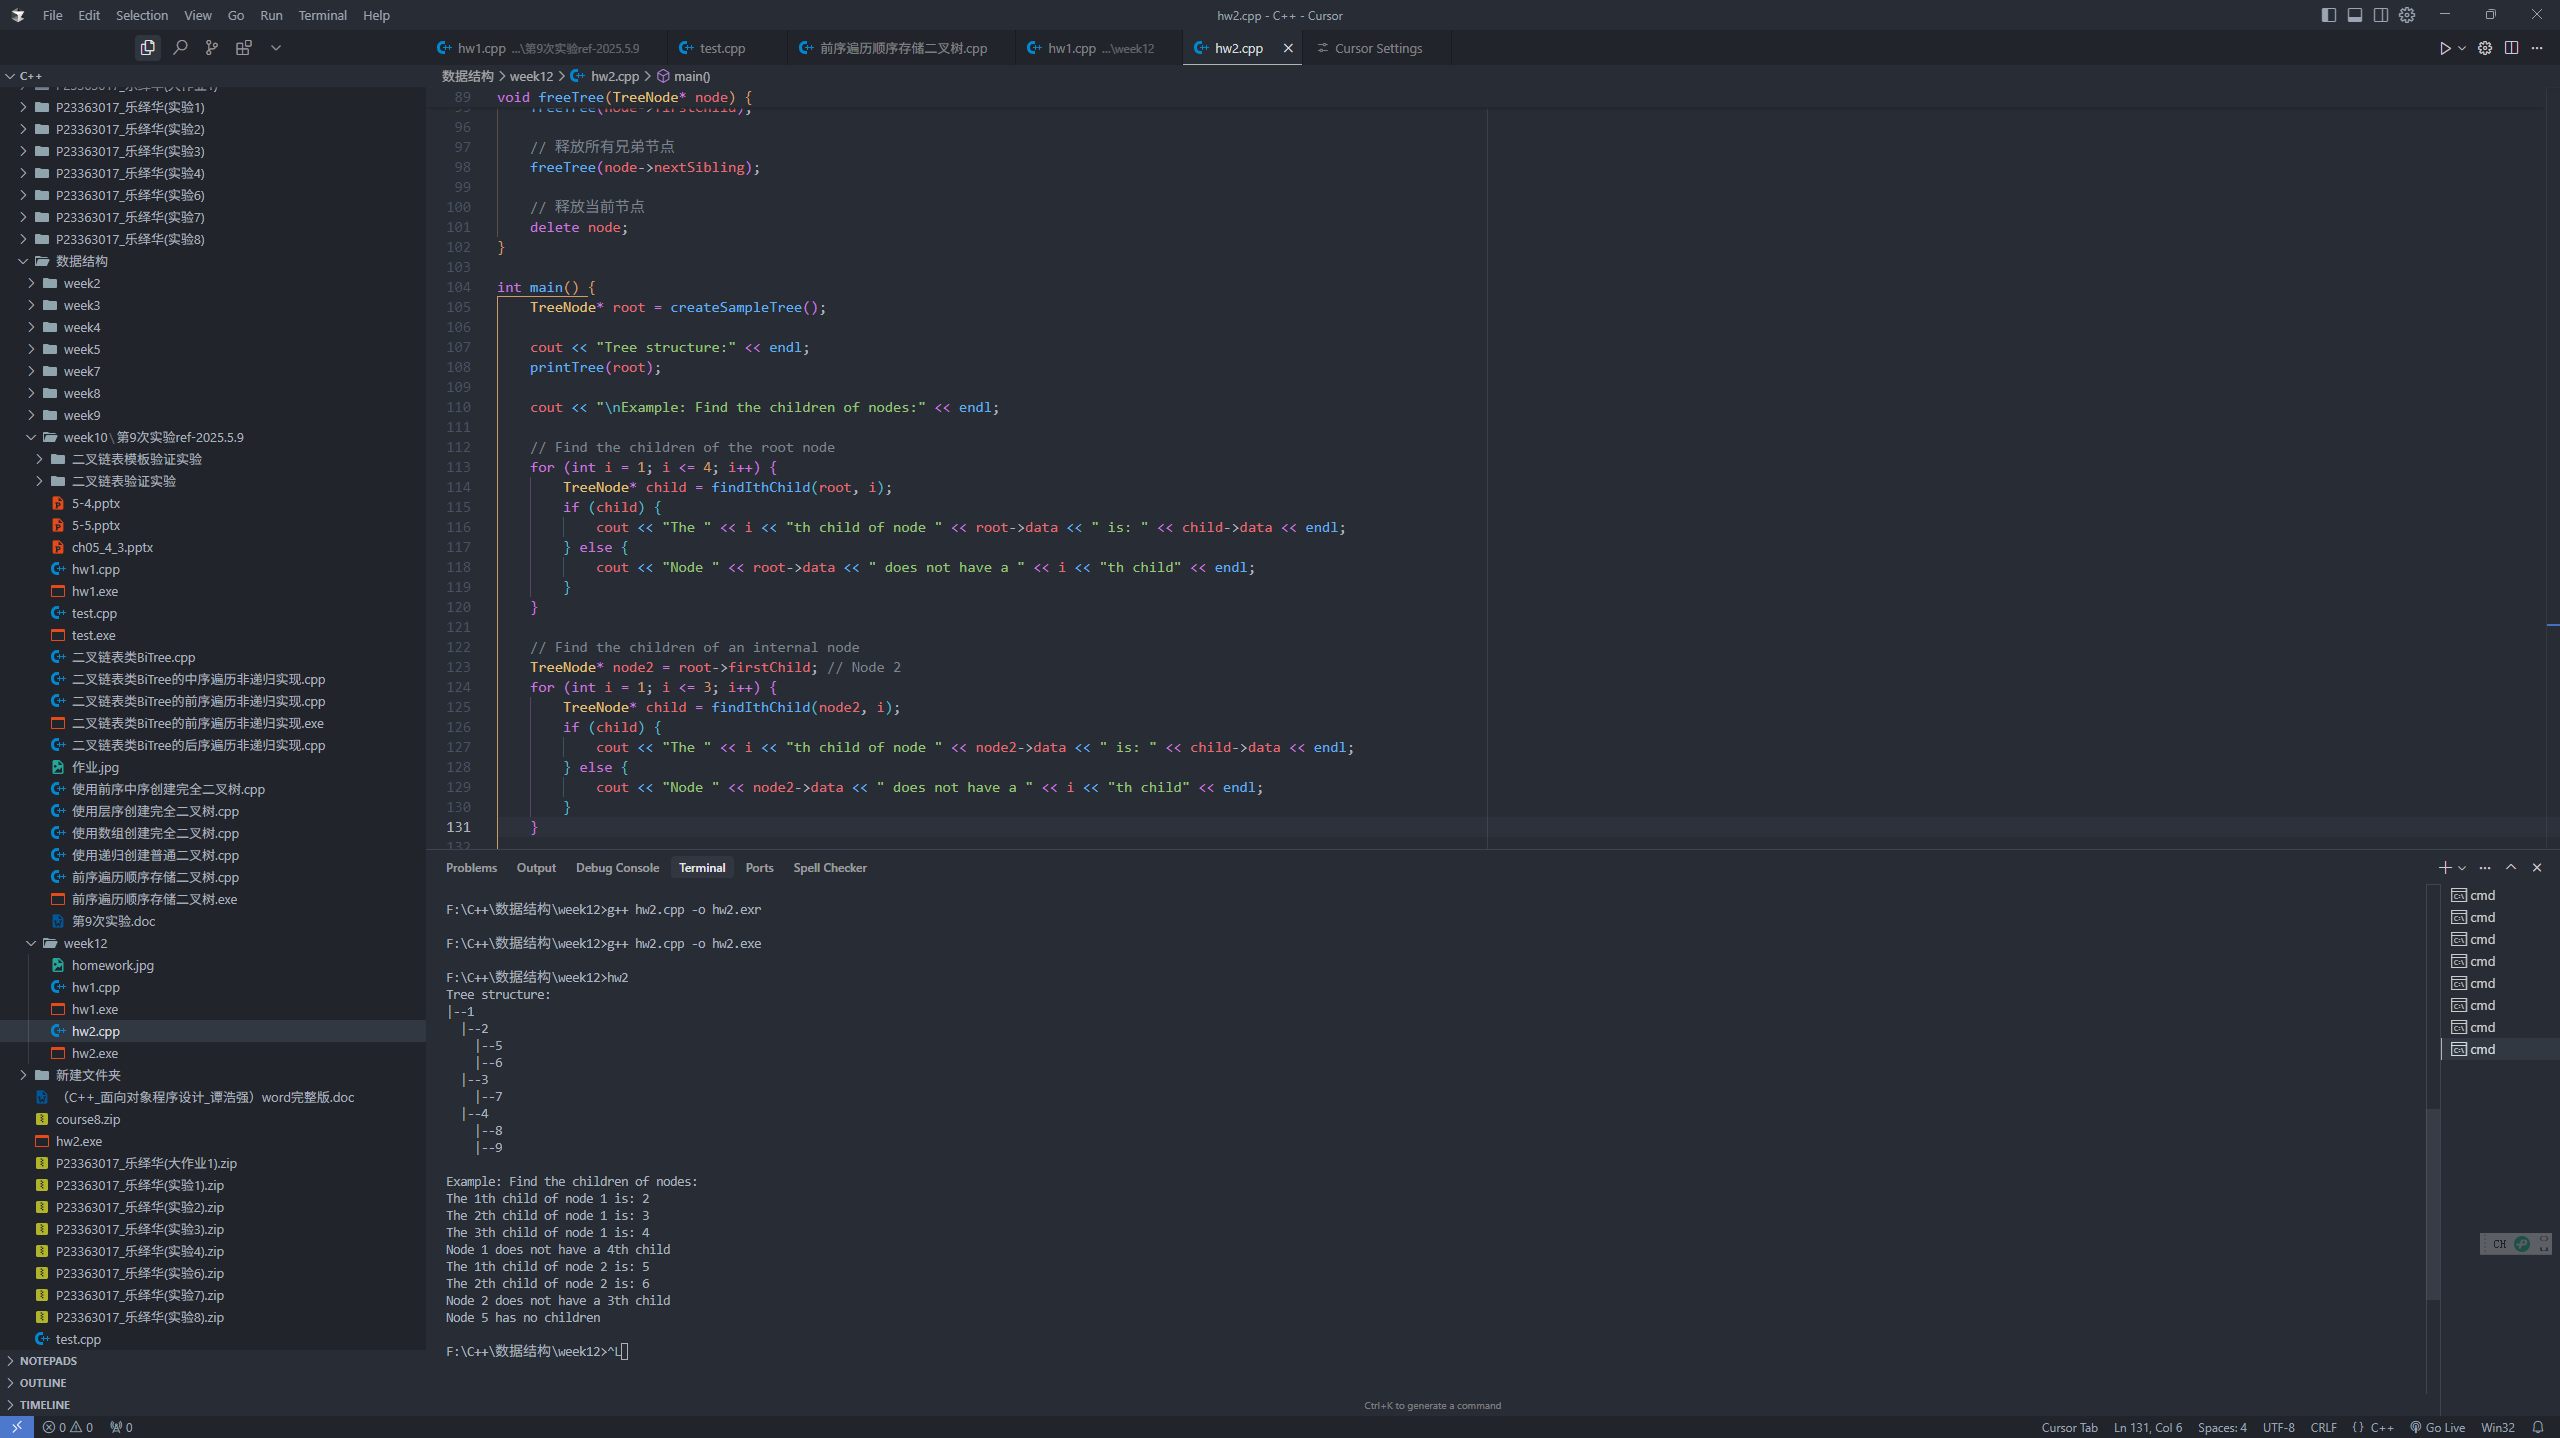
\includegraphics[width=\textwidth]{2-实验报告10-2025051923.png}
% \caption{}
\label{}
\end{figure}

\begin{lstlisting}[language=C++]

#include <iostream>

using namespace std;

  

// 树的结点结构 - 孩子兄弟表示法

struct TreeNode {

    int data;               // 结点数据

    TreeNode* firstChild;   // 指向第一个孩子

    TreeNode* nextSibling;  // 指向下一个兄弟

    TreeNode(int val) : data(val), firstChild(nullptr), nextSibling(nullptr) {}

};

  

// 查找结点x的第i个孩子(i从1开始计数)

TreeNode* findIthChild(TreeNode* x, int i) {

    if (x == nullptr || i < 1) {

        return nullptr;

    }

    // 找到第一个孩子

    TreeNode* child = x->firstChild;

    if (child == nullptr) {

        return nullptr; // 没有孩子

    }

    // 查找第i个孩子

    int count = 1;

    while (count < i && child != nullptr) {

        child = child->nextSibling;

        count++;

    }

    // 如果count等于i,说明找到了第i个孩子

    if (count == i) {

        return child;

    } else {

        return nullptr; // 孩子数量少于i

    }

}

  

// 创建一棵示例树

TreeNode* createSampleTree() {

    /*

           1

         / | \

        2  3  4

       /|  |  |\

      5 6  7  8 9

    */

    TreeNode* root = new TreeNode(1);

    // 第一层子结点

    root->firstChild = new TreeNode(2);

    root->firstChild->nextSibling = new TreeNode(3);

    root->firstChild->nextSibling->nextSibling = new TreeNode(4);

    // 第二层子结点

    root->firstChild->firstChild = new TreeNode(5);

    root->firstChild->firstChild->nextSibling = new TreeNode(6);

    root->firstChild->nextSibling->firstChild = new TreeNode(7);

    root->firstChild->nextSibling->nextSibling->firstChild = new TreeNode(8);

    root->firstChild->nextSibling->nextSibling->firstChild->nextSibling = new TreeNode(9);

    return root;

}

  

// 打印树结构(前序遍历)

void printTree(TreeNode* node, int level = 0) {

    if (node == nullptr) {

        return;

    }

    // 打印当前结点

    for (int i = 0; i < level; i++) {

        cout << "  ";

    }

    cout << "|--" << node->data << endl;

    // 递归打印所有子节点

    printTree(node->firstChild, level + 1);

    // 递归打印所有兄弟节点

    printTree(node->nextSibling, level);

}

  

// 释放树内存

void freeTree(TreeNode* node) {

    if (node == nullptr) {

        return;

    }

    // 释放所有子节点

    freeTree(node->firstChild);

    // 释放所有兄弟节点

    freeTree(node->nextSibling);

    // 释放当前节点

    delete node;

}

  

int main() {

    TreeNode* root = createSampleTree();

  

    cout << "Tree structure:" << endl;

    printTree(root);

  

    cout << "\nExample: Find the children of nodes:" << endl;

  

    // Find the children of the root node

    for (int i = 1; i <= 4; i++) {

        TreeNode* child = findIthChild(root, i);

        if (child) {

            cout << "The " << i << "th child of node " << root->data << " is: " << child->data << endl;

        } else {

            cout << "Node " << root->data << " does not have a " << i << "th child" << endl;

        }

    }

  

    // Find the children of an internal node

    TreeNode* node2 = root->firstChild; // Node 2

    for (int i = 1; i <= 3; i++) {

        TreeNode* child = findIthChild(node2, i);

        if (child) {

            cout << "The " << i << "th child of node " << node2->data << " is: " << child->data << endl;

        } else {

            cout << "Node " << node2->data << " does not have a " << i << "th child" << endl;

        }

    }

  

    // Find the children of a leaf node

    TreeNode* leaf = root->firstChild->firstChild; // Node 5

    TreeNode* child = findIthChild(leaf, 1);

    if (child) {

        cout << "The 1st child of node " << leaf->data << " is: " << child->data << endl;

    } else {

        cout << "Node " << leaf->data << " has no children" << endl;

    }

  

    // Free memory

    freeTree(root);

  

    return 0;

}


\end{lstlisting}
\section{3. 哈夫曼算法的应用}

假设某文本文档只包含26 个英文字母,应用哈夫曼算法对该文档进行压缩和解压缩操作,分析实际压缩比。

\begin{figure}[H]
\centering
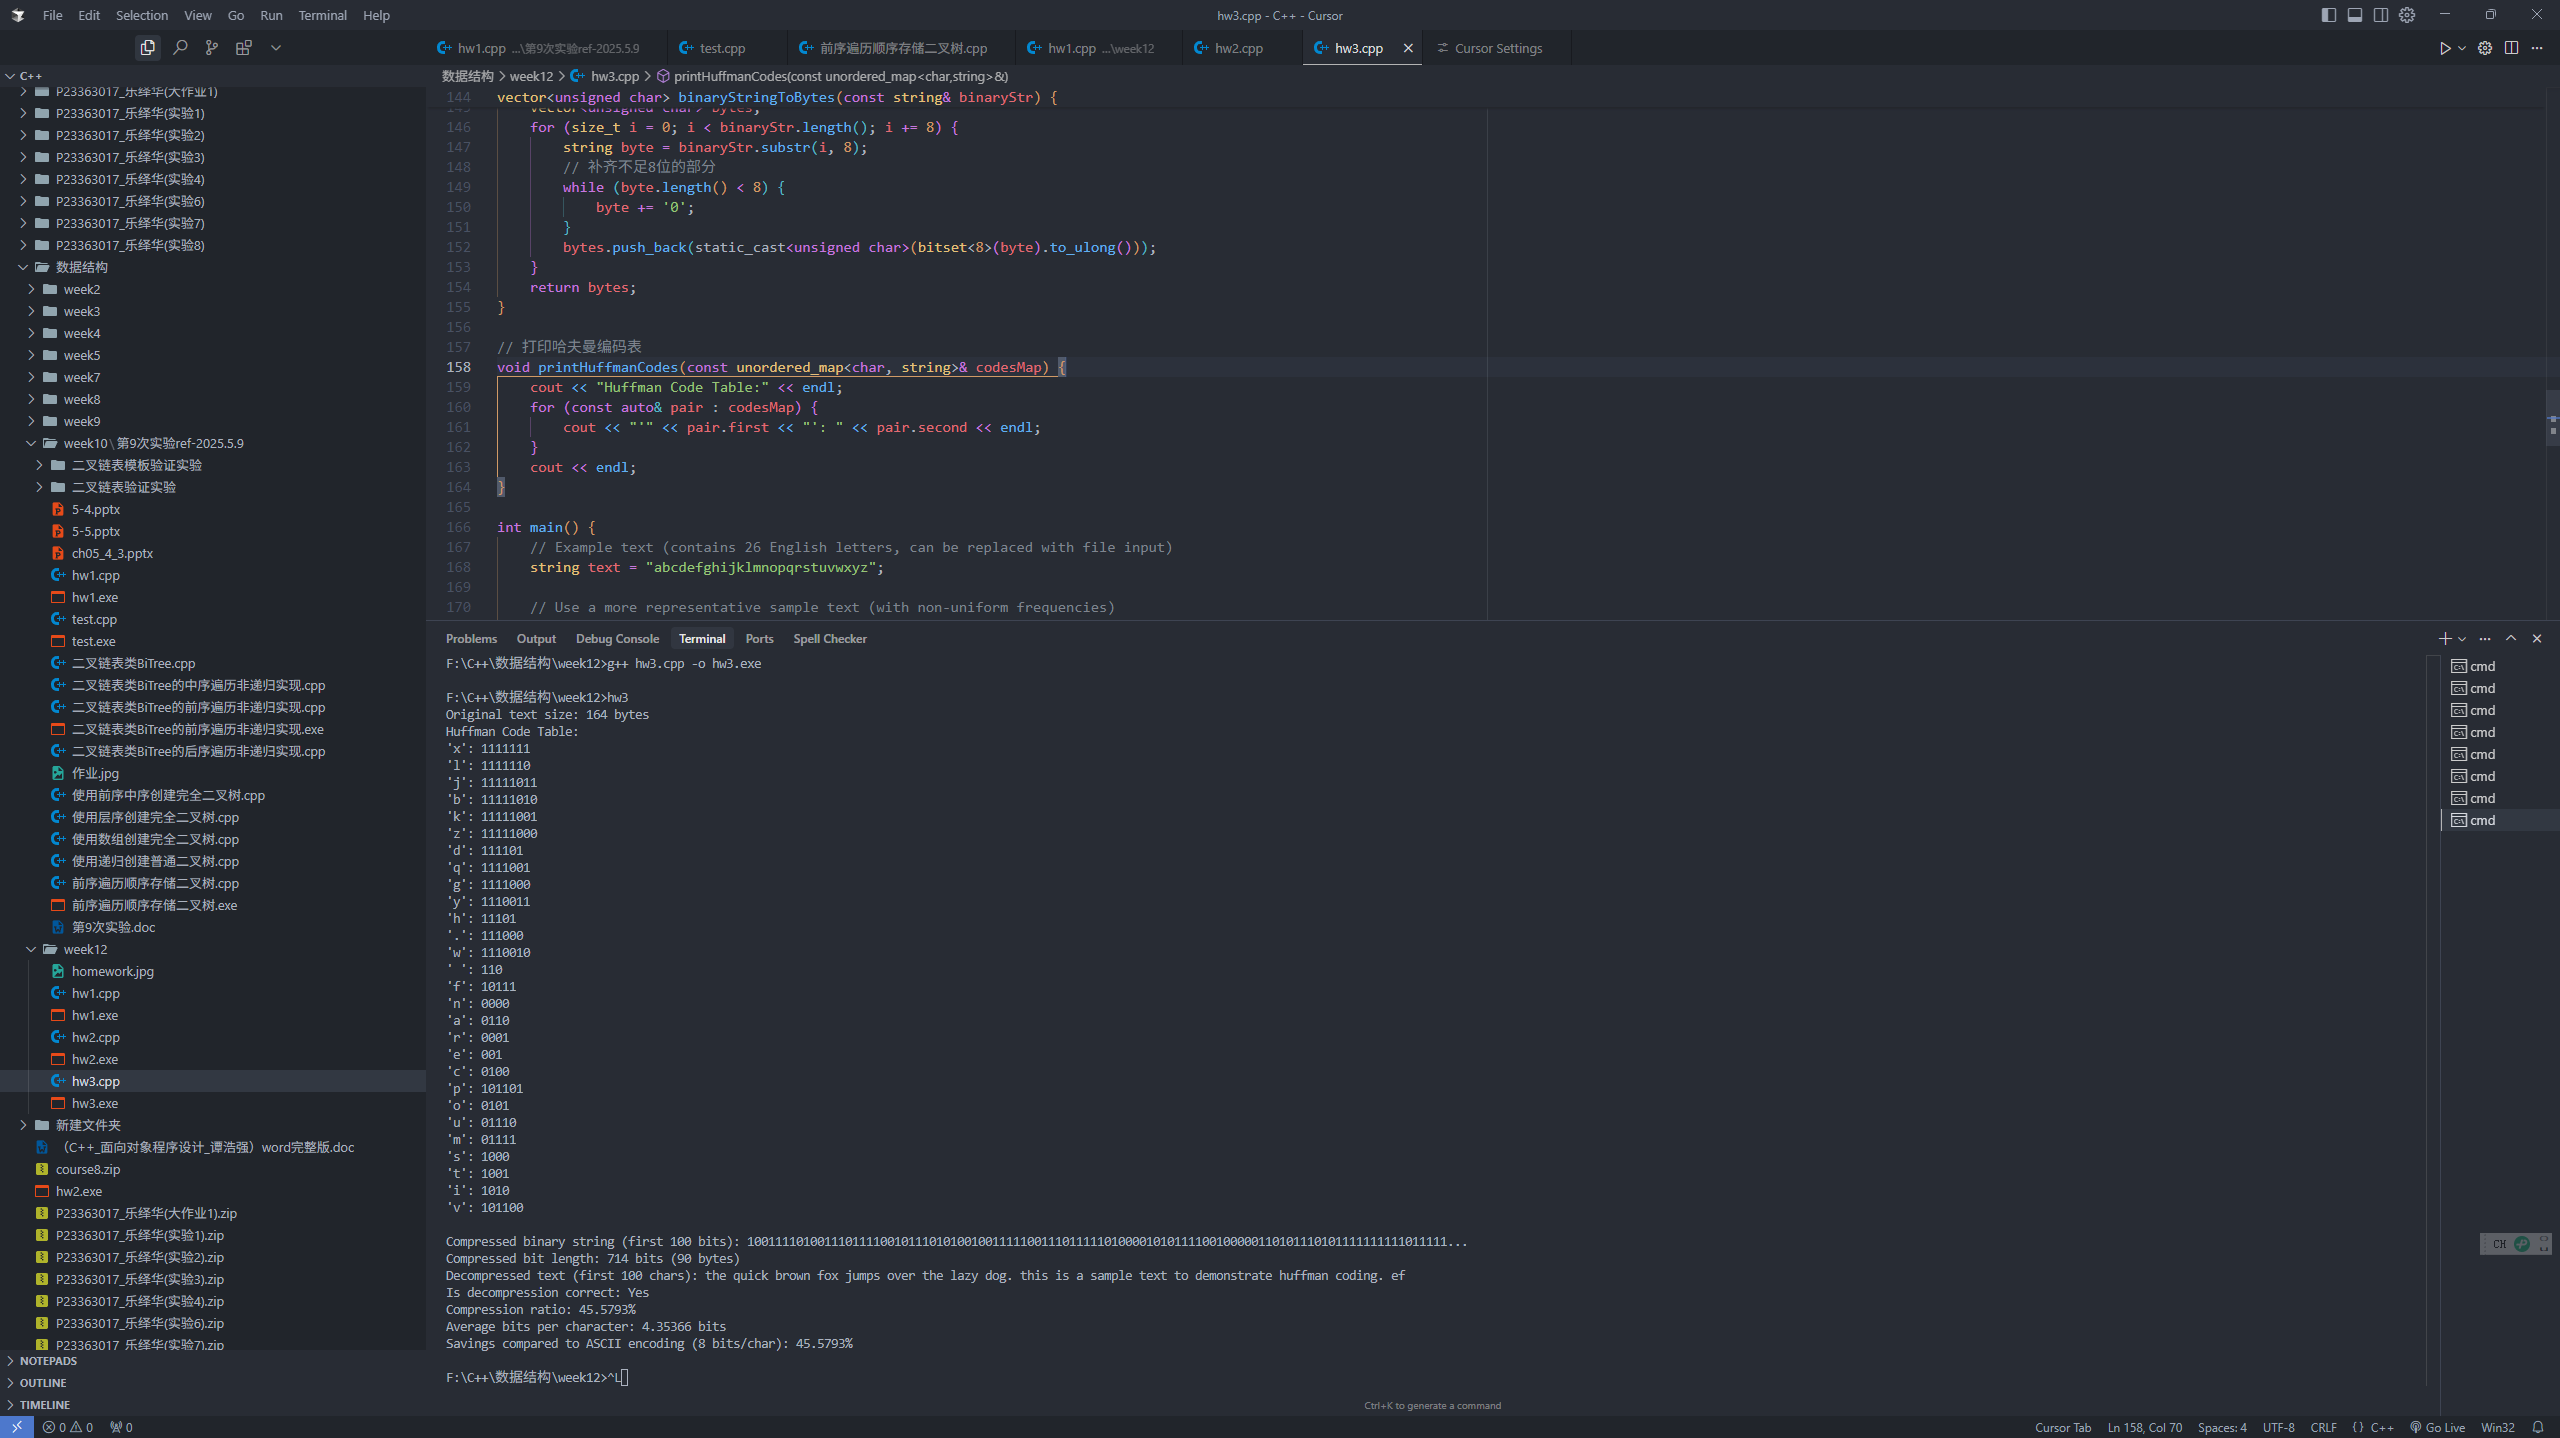
\includegraphics[width=\textwidth]{3-实验报告10-2025051923.png}
% \caption{}
\label{}
\end{figure}

\begin{lstlisting}[language=C++]
#include <iostream>

#include <fstream>

#include <string>

#include <queue>

#include <unordered_map>

#include <bitset>

#include <vector>

using namespace std;

  

// 哈夫曼树的结点结构

struct HuffmanNode {

    char data;              // 字符

    int frequency;          // 频率

    HuffmanNode* left;      // 左子结点

    HuffmanNode* right;     // 右子结点

    // 构造函数

    HuffmanNode(char data, int freq) :

        data(data), frequency(freq), left(nullptr), right(nullptr) {}

    // 比较用于优先队列

    bool operator>(const HuffmanNode& other) const {

        return frequency > other.frequency;

    }

};

  

// 自定义比较函数,用于优先队列

struct CompareNodes {

    bool operator()(HuffmanNode* a, HuffmanNode* b) {

        return a->frequency > b->frequency;

    }

};

  

// 计算字符频率

unordered_map<char, int> calculateFrequency(const string& text) {

    unordered_map<char, int> freqMap;

    for (char c : text) {

        freqMap[c]++;

    }

    return freqMap;

}

  

// 构建哈夫曼树

HuffmanNode* buildHuffmanTree(const unordered_map<char, int>& freqMap) {

    // 使用优先队列(小顶堆)

    priority_queue<HuffmanNode*, vector<HuffmanNode*>, CompareNodes> pq;

    // 将所有叶子结点加入优先队列

    for (const auto& pair : freqMap) {

        pq.push(new HuffmanNode(pair.first, pair.second));

    }

    // 构建哈夫曼树

    while (pq.size() > 1) {

        // 取出频率最小的两个结点

        HuffmanNode* left = pq.top(); pq.pop();

        HuffmanNode* right = pq.top(); pq.pop();

        // 创建新的内部结点,频率为两个子结点的和

        HuffmanNode* newNode = new HuffmanNode('\0', left->frequency + right->frequency);

        newNode->left = left;

        newNode->right = right;

        // 将新结点放回优先队列

        pq.push(newNode);

    }

    // 返回树的根结点

    return pq.top();

}

  

// 生成哈夫曼编码

void generateCodes(HuffmanNode* root, const string& code,

                  unordered_map<char, string>& codesMap) {

    if (root == nullptr) {

        return;

    }

    // 如果是叶子结点,添加编码到map

    if (root->left == nullptr && root->right == nullptr) {

        codesMap[root->data] = code;

    }

    // 递归左子树,编码添加'0'

    generateCodes(root->left, code + "0", codesMap);

    // 递归右子树,编码添加'1'

    generateCodes(root->right, code + "1", codesMap);

}

  

// 压缩文本

string compressText(const string& text, const unordered_map<char, string>& codesMap) {

    string compressed;

    for (char c : text) {

        compressed += codesMap.at(c);

    }

    return compressed;

}

  

// 解压缩文本

string decompressText(const string& compressed, HuffmanNode* root) {

    string decompressed;

    HuffmanNode* current = root;

    for (char bit : compressed) {

        // 根据位值选择左右分支

        if (bit == '0') {

            current = current->left;

        } else if (bit == '1') {

            current = current->right;

        }

        // 如果到达叶子结点,添加字符到结果,并重新从根开始

        if (current->left == nullptr && current->right == nullptr) {

            decompressed += current->data;

            current = root;

        }

    }

    return decompressed;

}

  

// 释放哈夫曼树内存

void freeHuffmanTree(HuffmanNode* root) {

    if (root == nullptr) {

        return;

    }

    freeHuffmanTree(root->left);

    freeHuffmanTree(root->right);

    delete root;

}

  

// 计算压缩比

double calculateCompressionRatio(const string& original, const string& compressed) {

    // 原始文本每个字符占8位

    double originalSize = original.length() * 8;

    double compressedSize = compressed.length();

    return (originalSize - compressedSize) / originalSize * 100.0;

}

  

// 将压缩后的二进制字符串转为字节串

vector<unsigned char> binaryStringToBytes(const string& binaryStr) {

    vector<unsigned char> bytes;

    for (size_t i = 0; i < binaryStr.length(); i += 8) {

        string byte = binaryStr.substr(i, 8);

        // 补齐不足8位的部分

        while (byte.length() < 8) {

            byte += '0';

        }

        bytes.push_back(static_cast<unsigned char>(bitset<8>(byte).to_ulong()));

    }

    return bytes;

}

  

// 打印哈夫曼编码表

void printHuffmanCodes(const unordered_map<char, string>& codesMap) {

    cout << "Huffman Code Table:" << endl;

    for (const auto& pair : codesMap) {

        cout << "'" << pair.first << "': " << pair.second << endl;

    }

    cout << endl;

}

  

int main() {

    // Example text (contains 26 English letters, can be replaced with file input)

    string text = "abcdefghijklmnopqrstuvwxyz";

    // Use a more representative sample text (with non-uniform frequencies)

    text = "the quick brown fox jumps over the lazy dog. "

           "this is a sample text to demonstrate huffman coding. "

           "efficient compression is achieved when character frequencies vary.";

    cout << "Original text size: " << text.length() << " bytes" << endl;

    // Calculate character frequencies

    unordered_map<char, int> freqMap = calculateFrequency(text);

    // Build Huffman tree

    HuffmanNode* root = buildHuffmanTree(freqMap);

    // Generate Huffman codes

    unordered_map<char, string> codesMap;

    generateCodes(root, "", codesMap);

    // Print Huffman codes

    printHuffmanCodes(codesMap);

    // Compress the text

    string compressed = compressText(text, codesMap);

    cout << "Compressed binary string (first 100 bits): " << compressed.substr(0, 100) << "..." << endl;

    cout << "Compressed bit length: " << compressed.length() << " bits"

         << " (" << (compressed.length() + 7) / 8 << " bytes)" << endl;

    // Decompress the text

    string decompressed = decompressText(compressed, root);

    // Verify decompression result

    cout << "Decompressed text (first 100 chars): " << decompressed.substr(0, 100) << endl;

    cout << "Is decompression correct: " << (text == decompressed ? "Yes" : "No") << endl;

    // Calculate and display compression ratio

    double compressionRatio = calculateCompressionRatio(text, compressed);

    cout << "Compression ratio: " << compressionRatio << "%" << endl;

    // Analyze average code length per character

    double totalBits = 0;

    int totalChars = 0;

    for (const auto& pair : freqMap) {

        totalBits += pair.second * codesMap[pair.first].length();

        totalChars += pair.second;

    }

    double avgBitsPerChar = totalBits / totalChars;

    cout << "Average bits per character: " << avgBitsPerChar << " bits" << endl;

    cout << "Savings compared to ASCII encoding (8 bits/char): "

         << (8 - avgBitsPerChar) / 8 * 100 << "%" << endl;

    // Free Huffman tree memory

    freeHuffmanTree(root);

    return 0;

}
\end{lstlisting}